\section{Разработка и оформления элементов управления}
\graphicspath{{parts/guides/3_controls/images/}}

\subsection{Классы \mintinline{csharp}{Brush}, \mintinline{csharp}{Pen}}

\subsubsection{Класс \mintinline{csharp}{Brush}, градиентная заливка}

В примерах ранее были упомянуты такие свойства, как \mintinline{xml}{Background} и \mintinline{xml}{Foreground} и назначение им определенного цвета. Но если посмотреть чуть глубже, то для установки цвета нам нужен объект класса \mintinline{csharp}{System.Media.Brush}. Значение \mintinline{xml}{"Blue"} в данном случае является свойством класса \mintinline{xml}{Brushes}, которое инкапсулирует объект \mintinline{csharp}{SolidColorBrush}. Например, в C\texttt{\#} коде мы можем установить цвет так \mintinline{csharp}{SomeButton.Background = Brushes.Blue}.

Класс \mintinline{csharp}{SolidColorBrush} является кистью или наследником класса \mintinline{csharp}{Brush}, с помощью которого, таким образом, можно устанавливать свойства \mintinline{xml}{Background}, \mintinline{xml}{Foreground} и \mintinline{xml}{BorderBrush}.

WPF поддерживает целый ряд кистей

\begin{description}[style=nextline]
\item [\mintinline{xml}{SolidColorBrush}] Заливает содержимое сплошным цветом.

\begin{minted}{xml}
<Button  Width="160" Height="30" Content="SolidColorBrush">
    <Button.FontSize>18</Button.FontSize>
    <Button.Background>
        <SolidColorBrush Color="Blue" Opacity="0.8" />
    </Button.Background>
    <Button.Foreground>
        <SolidColorBrush Color="White"/>
    </Button.Foreground>
</Button>
\end{minted}

С помощью code-behind кода кисть можно использовать так

\begin{minted}{csharp}
SomeButton.Background = new SolidColorBrush(Colors.Blue);
AnotherOneButton.Background = new SolidColorBrush(Color.FromRgb(207, 255, 255));
\end{minted}

\item [\mintinline{xml}{LinearGradientBrush}] Эта кисть создает плавный переход от одного цвета к другому. Для указания цвета и точек, от которых начинается переход, используется объект GradientStop. Его свойство Color указывает на цвет, а свойство Offset- на точку, с которой начинается переход.

\begin{minted}{xml}
<Button Width="200" Height="50" Content="LinearGradientBrush" >
    <Button.FontSize>18</Button.FontSize>
    <Button.Background>
        <LinearGradientBrush StartPoint="0.5,1" EndPoint="0.5,0">
            <GradientStop Color="White" Offset="0" />
            <GradientStop Color="DarkOrange" Offset="1" />
        </LinearGradientBrush>
    </Button.Background>
    <Button.Foreground>
        <LinearGradientBrush>
            <GradientStop Color="Blue" Offset="1" />
            <GradientStop Color="Green" Offset="0.5" />
            <GradientStop Color="Red" Offset="0" />
        </LinearGradientBrush>
    </Button.Foreground>
</Button>
\end{minted}

С помощью свойств \mintinline{xml}{StartPoint} и \mintinline{xml}{EndPoint} можно определить направление градиента, сделать горизонтальный градиент или градиент под углом.

\item [\mintinline{xml}{RadialGradientBrush}] Эта кисть заполняет элемент радиальным градиентом. Объект \mintinline{xml}{RadialGradientBrush} также имеет коллекцию объектов \mintinline{xml}{GradientStop}, задающих цвет и смещение. Кроме того, он позволяет задавать центр градиента с помощью свойства \mintinline{xml}{GradientOrigin}

\begin{minted}{xml}
<Button Width="200" Height="50" Content="RadialGradientBrush">
    <TextBlock.FontSize>18</TextBlock.FontSize>
    <Button.Background>
        <RadialGradientBrush GradientOrigin="0.4,0.1">
            <GradientStop Color="Black" Offset="1" />
            <GradientStop Color="Blue" Offset="0" />
        </RadialGradientBrush>
    </Button.Background>
    <Button.Foreground>
        <RadialGradientBrush Center="0.4,0.4"  SpreadMethod="Reflect">
            <GradientStop Color="Orange" Offset="1" />
            <GradientStop Color="Red" Offset="0.2" />
        </RadialGradientBrush>
    </Button.Foreground>
</Button>
\end{minted}

Также \mintinline{xml}{RadialGradientBrush} позволяет ограничить область градиента с помощью свойств \mintinline{xml}{RadiusX} и \mintinline{xml}{RadiusY}

\begin{minted}{xml}
<Ellipse Width="60" Height="60"  >
    <Ellipse.Fill>
        <RadialGradientBrush RadiusX="0.6" RadiusY="0.8" GradientOrigin="0.3,0.3">
            <GradientStop Color="Red" Offset="1" />
            <GradientStop Color="White" Offset="0" />
        </RadialGradientBrush>
    </Ellipse.Fill>
</Ellipse>
\end{minted}

\item [\mintinline{xml}{ImageBrush}] Эта кисть использует изображение в качестве фона. Источник устанавливается свойством \mintinline{xml}{ImageSource}. Свойство \mintinline{xml}{Stretch} задает способ заполнения элемента изображением. Если оно равно \mintinline{xml}{Fill} (по умолчанию), то изображение заполняет весь элемент, растягиваясь, если это нужно. Если \mintinline{xml}{Stretch="Uniform"}, то изображение масштабируется пропорционально размеру элемента и по краям могут образоваться пустые места, не заполненные изображением.

\begin{minted}{xml}
<Image Source="image.png" Stretch="Uniform"/>
\end{minted}

Среди прочих свойств \mintinline{xml}{ImageBrush} следует отметить свойство \mintinline{xml}{Viewbox}. Оно применяется для выреза какой-то части изображения. 

\begin{minted}{xml}
<Canvas>
    <Canvas.Background>
        <ImageBrush ImageSource="image.png" Stretch="Uniform"
                    Viewbox="0.5,0.45,0.3,0.2" 
        />
    </Canvas.Background>
</Canvas>
\end{minted}

Его первый параметр служит для установки x-координаты изображения, а второй параметр — y-координаты. Они находятся в пределах от \mintinline{xml}{0} до \mintinline{xml}{1}, и чтобы получить реальные координаты изображения, надо умножить первый параметр на ширину, а второй параметр — на высоту изображения. Третий и четвертый параметр указывают соответственно на ширину и высоту вырезаемого изображения. Так ниже в примере, начальная точка выреза изображения имеет координаты: \mintinline{xml}{0.5 * ширина_изображения}, \mintinline{xml}{0.45 * высота_изображения}. Вырезается 30\% от оставшейся ширины и 20\% от оставшейся длины.

\mintinline{xml}{ImageBrush} также позволяет нам многократно отобразить изображение на элементе и проделывать с ним некоторые преобразования. Для этого класс \mintinline{xml}{ImageBrush} имеет свойство \mintinline{xml}{Viewport}. Оно похоже на \mintinline{xml}{Viewbox}, также задает четыре параметра, только они указывают на координаты прямоугольника \mintinline{xml}{Viewbox} на элементе управления. Первый и второй параметр указывают на начальную координату этого прямоугольника, а третий и четвертый — на конечную точку. Реальные координаты получаются путем умножения параметров на длину и ширину элемента.

Кроме того, свойство \mintinline{xml}{TileMode} позволяет задать режим заполнения элемента изображением. Оно имеет четыре варианта:

\begin{description}[style=nextline]
\item [\mintinline{xml}{Tile}] Изображение многократно повторяется на элементе, пока не заполнит все пространство.
\item [\mintinline{xml}{FlipX}] Изображение повторяется по оси X, и каждый второй столбец является зеркальным отображением предыдущего.
\item [\mintinline{xml}{FlipY}] Изображение повторяется по оси Y, и каждая вторая строка является зеркальным отображением предыдущей.
\item [\mintinline{xml}{FlipXY}] Каждое изображение зеркально отображается как по оси Х, так и по оси Y.
\item [\mintinline{xml}{None}] Создается единичное изображение (по умолчанию)
\end{description}

Пример использования \mintinline{xml}{TileMode}
\begin{minted}{xml}
<Grid.Background>
    <ImageBrush ImageSource="D:\Images\Image.jpg"
                Viewport="0,0,0.25,0.25" TileMode="FlipXY" />
</Grid.Background>
\end{minted}

\item [\mintinline{xml}{DrawingBrush}] С помощью свойства \mintinline{xml}{Drawing} определяет рисунок, включающий: геометрические фигуры, другие элементы и т.д., служащее заполнителем. Он использует те же свойства, что и \mintinline{xml}{ImageBrush}: \mintinline{xml}{Viewport} и \mintinline{xml}{Viewbox}.

\mintinline{xml}{ImageDrawing} — заполнителем кисти является изображение.

\mintinline{xml}{GeometryDrawing} — кисть формируется на основе рисунка, составленного каким-нибудь геометрическим примитивом (прямоугольником, линией, эллипсом)

\mintinline{xml}{VideoDrawing} — кисть формируется на основе видеоресурса.

\mintinline{xml}{GlyphRunDrawing}

При необходимости сочетания нескольких вариантов, используется свойство \mintinline{xml}{DrawingGroup} класса \mintinline{xml}{Drawing}.

\begin{minted}{xml}
<DrawingBrush TileMode="FlipXY" Viewport="0,0,0.25,0.25">
    <DrawingBrush.Drawing>
        <DrawingGroup>
            <GeometryDrawing Brush="Aquamarine">
                <GeometryDrawing.Pen>
                    <Pen Brush="Black" />
                </GeometryDrawing.Pen>
                <GeometryDrawing.Geometry>
                    <EllipseGeometry RadiusX="30" RadiusY="30" 
                                     Center="150,125" />
                </GeometryDrawing.Geometry>
            </GeometryDrawing>
            <GeometryDrawing Brush="Aquamarine">
                <GeometryDrawing.Pen>
                    <Pen Brush="Black" />
                </GeometryDrawing.Pen>
                <GeometryDrawing.Geometry>
                    <LineGeometry EndPoint="150,125" />
                </GeometryDrawing.Geometry>
            </GeometryDrawing>
        </DrawingGroup>
    </DrawingBrush.Drawing>
</DrawingBrush>
\end{minted}

\item [\mintinline{xml}{VisualBrush}] Эта кисть при помощи свойства \mintinline{xml}{Visual} создает привязку к определенному элементу, копируя весь его фон или его часть.

VisualBrush, как и кисти \mintinline{xml}{DrawingBrush} и \mintinline{xml}{ImageBrush}, обладает свойствами \mintinline{xml}{Viewport}, \mintinline{xml}{Viewbox} и \mintinline{xml}{TileMode}, позволяющие проводить все те же преобразования, что были рассмотрены для этих кистей

\begin{minted}{xml}
<Grid Background="Lavender">
    <Button Name="SomeButton" Content="VisualBrush" 
            Background="Black" FontWeight="Black" Foreground="White" 
            HorizontalAlignment="Center" VerticalAlignment="Top"
            Width="100" Height="30"/>
    <TextBlock HorizontalAlignment="Center" VerticalAlignment="Center"
               Width="120" Height="35">
        <TextBlock.Background>
            <VisualBrush Visual="{Binding ElementName=SomeButton}" />
        </TextBlock.Background>
    </TextBlock>
    <TextBlock HorizontalAlignment="Center" VerticalAlignment="Bottom"
               Width="140" Height="50">
        <TextBlock.Background>
            <VisualBrush Visual="{Binding ElementName=SomeButton}" 
                         Viewbox="0.1,0.1,0.3,0.7" />
        </TextBlock.Background>
    </TextBlock>
</Grid>
\end{minted}

\end{description}

Использования различных вариантов кистей:
\begin{figure}[H]
\centering
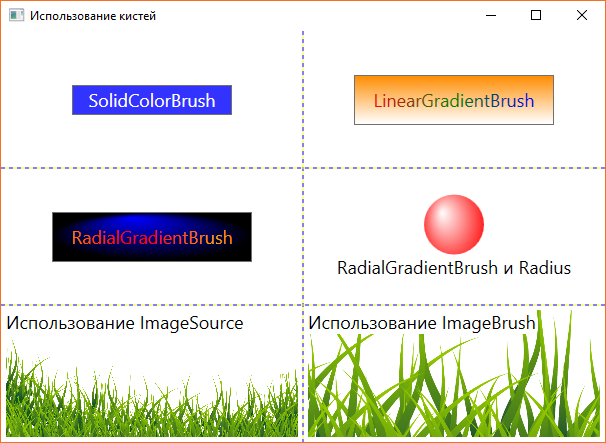
\includegraphics[width=1\textwidth]{brushes.png}
\end{figure}


\newpage
\subsubsection{Класс \mintinline{xml}{Pen}}

В параграфе выше мы так же использовали класс \mintinline{xml}{Pen}. При его использовании мы указывали свойства \mintinline{xml}{Brush} и \mintinline{xml}{Thickness}, что позволяло описывать способ рисования контура фигуры. Но в классе \mintinline{xml}{Pen} определены и другие свойства для более точного управления внешним видом

\begin{description}[style=nextline]

\item [\mintinline{xml}{StartLineCap} и \mintinline{xml}{EndLineCap}] Описывает открытый конец отрезка и может принимать значения, определенные в перечислении \mintinline{xml}{PenLineCap}: \mintinline{xml}{Flat} (плоский, по умолчанию), \mintinline{xml}{Square}, \mintinline{xml}{Round} и \mintinline{xml}{Triangle}. Вид линии в точке соединения двух отрезков управляется свойством \mintinline{xml}{LineJoin}.

\item [\mintinline{xml}{LineJoin}] Описывает способ соединения отрезков в углах ломаной. Может принимать значения из перечисления \mintinline{xml}{PenLineJoin}: \mintinline{xml}{Miter} (по умолчанию), \mintinline{xml}{Round} и \mintinline{xml}{Bevel}. Отдельное свойство \mintinline{xml}{MiterLimit} определяет, насколько выступает уголок соединения типа \mintinline{xml}{Miter}. Если эту длину не ограничить, то для острых углов выступ может оказаться очень большим. По умолчанию принимается значение \mintinline{xml}{10}.

\item [\mintinline{xml}{DashStyle}] Описывает стили линии, рисуемой пером (она необязательно сплошная). Значением этого свойства должен быть объект типа \mintinline{xml}{DashStyle}. Начертание конечных точек штриха можно регулировать свойством \mintinline{xml}{DashCap} класса \mintinline{xml}{Реп}. Оно аналогично свойствам \mintinline{xml}{StartLineCap} и \mintinline{xml}{EndLineCap}, только по умолчанию равно \mintinline{xml}{Square}, а не \mintinline{xml}{Flat}.

\end{description}


Рассмотрим подробнее класс \mintinline{xml}{DashStyle}. В нем имеется свойство \mintinline{xml}{Dashes}. Это простая коллекция \mintinline{xml}{DoubleCollection}, в которой хранится последовательность чисел, представляющих длины штрихов и промежутков между ними. В нечетных элементах находятся длины штрихов (относительно толщины пера), а в четных — длины промежутков. Заданная последовательность повторяется до бесконечности. В классе \mintinline{xml}{DashStyle} имеется также свойство \mintinline{xml}{Offset} типа \mintinline{csharp}{double}, определяющее, где начинает рисоваться последовательность. Странность поведения \mintinline{xml}{DashStyle} заключается в том, что поскольку свойство \mintinline{xml}{DashCap} по умолчанию равно \mintinline{xml}{Square}, то штрих получается длиннее промежутка с точно таким же числовым значением. Более того, для длины штриха вполне можно задать значение \mintinline{xml}{0}, и тогда она окажется равной толщине пера. 

Имеется еще класс \mintinline{xml}{DashStyles}, и в его статическом свойстве \mintinline{xml}{DashStyle} определены некоторые типичные варианты начертания штрихпунктирных линий. Например, можно выбрать вариант \mintinline{xml}{DashDotDot}

\begin{minted}{xml}
<Pen Brush="Black" Thickness="10" DashStyle="{x:Static DashStyles.DashDotDot}" />
\end{minted}

\newpage
\begin{minted}{xml}
<Image>
<Image.Source>
    <DrawingImage>
        <DrawingImage.Drawing>
            <DrawingGroup>
                <!-- Тело -->
                <GeometryDrawing Brush="Orange" Geometry="
                    M 240,250
                    C 200,375 200,250 175,200
                    C 100,400 100,250 100,200
                    C 0,350 0,250 30,130
                    C 75,0 100,0 150,0
                    C 200,0 250,0 250,150 Z"/>
                
                <!-- Глаза -->
                <GeometryDrawing Brush="Black">
                    <GeometryDrawing.Pen>
                        <Pen Brush="White" Thickness="10"/>
                    </GeometryDrawing.Pen>
                    <GeometryDrawing.Geometry>
                        <GeometryGroup>
                            <!-- Левый глаз -->
                            <EllipseGeometry RadiusX="15" RadiusY="15" Center="95,95"/>
                            <!-- Правый глаз -->
                            <EllipseGeometry RadiusX="15" RadiusY="15" Center="170,105"/>
                        </GeometryGroup>
                    </GeometryDrawing.Geometry>
                </GeometryDrawing>
                
                <!-- Рот-->
                <GeometryDrawing>
                    <GeometryDrawing.Pen>
                        <Pen Brush="Black" StartLineCap="Round" EndLineCap="Round" 
                        Thickness="10"/>
                    </GeometryDrawing.Pen>
                    <GeometryDrawing.Geometry>
                        <LineGeometry StartPoint="75,160" EndPoint="175,150"/>
                    </GeometryDrawing.Geometry>
                </GeometryDrawing>
            </DrawingGroup>
        </DrawingImage.Drawing>
    </DrawingImage>
</Image.Source>
</Image>
\end{minted}

\newpage
Полученный результат:
\begin{figure}[H]
\centering
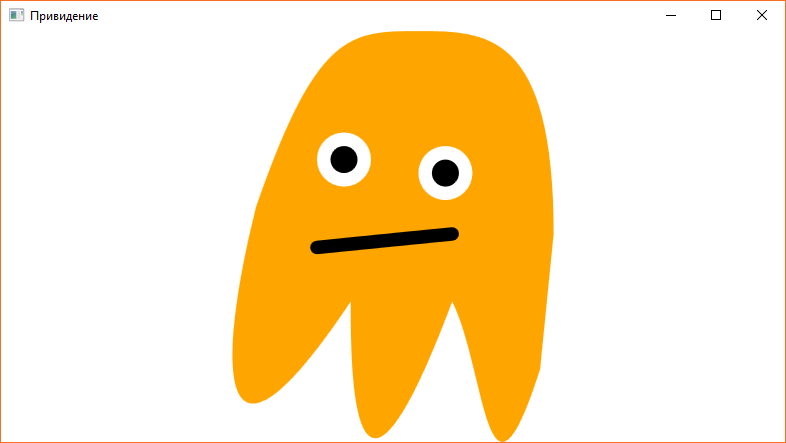
\includegraphics[width=0.75\textwidth]{ghost.png}
\end{figure}

\subsection{Ресурсы}

\subsubsection{Общая концепция}
В .NET Framework встроена общая инфраструктура пакетирования и доступа к ресурсам — частям приложения или компонента, отличным от кода. К ним относятся, например, растровые изображения, шрифты, аудио и видеофайлы и тому подобное. Как и во многих других случаях, WPF не только пользуется базовой системой ресурсов .NET, но и немного расширяет ее. В WPF поддерживается два разных вида ресурсов: бинарные и логические. Мы разберем логические, так как они нам наиболее интересны.

В чем смысл использования ресурсов? Они повышают эффективность: мы можем определить один раз какой-либо ресурс и затем многократно использовать его в различных местах приложения. В связи с этим улучшается поддержка - если возникнет необходимость изменить ресурс, достаточно это сделать в одном месте, и изменения произойдут глобально в приложении.

Логические ресурсы представляют собой произвольные объекты .NET, хранящиеся в свойстве элемента \mintinline{xml}{Resources}. Обычно предполагается, что таким ресурсом смогут сообща пользоваться все потомки данного элемента. Свойство \mintinline{xml}{Resources}  определено в базовых классах \mintinline{xml}{FrameworkElement} и \mintinline{xml}{FrameworkContentElement}, а занчит, оно есть в большинстве классов WPF. В качетсве таких ресурсов часто выступает стили, либо поставщики данных.

Рассмотрим простой пример, показывающий удобство использования логических ресурсов. Предположим нам нужно создать панель с 5 кнопками. Каждая кнопка должна быть желтой, с красной обводкой и белым текстом. Тогда решение без использования ресурсов будет выглядеть так:

\newpage
\begin{minted}{xml}
<Window x:Class="HelloWorldApp.MainWindow"
        xmlns="http://schemas.microsoft.com/winfx/2006/xaml/presentation"
        xmlns:x="http://schemas.microsoft.com/winfx/2006/xaml"
        xmlns:d="http://schemas.microsoft.com/expression/blend/2008"
        xmlns:mc="http://schemas.openxmlformats.org/markup-compatibility/2006"
        xmlns:local="clr-namespace:HelloWorldApp"
        mc:Ignorable="d"
        Title="MainWindow" Height="450" Width="620">

    <Grid>
        <DockPanel Background="SteelBlue">
            <StackPanel 
                DockPanel.Dock="Top" Orientation="Horizontal" 
                HorizontalAlignment="Center" Margin="10" >
                <Button
                    MinWidth="100" Content="Test 1" 
                    BorderBrush="Red" BorderThickness="3"
                    Background="Orange" Foreground="White"
                    FontWeight="Bold" />
                <Button
                    MinWidth="100" Content="Test 2" 
                    BorderBrush="Red" BorderThickness="3"
                    Background="Orange" Foreground="White"
                    FontWeight="Bold" />
                    
                <Button 
                    MinWidth="100" Content="Test 3" 
                    BorderBrush="Red" BorderThickness="3"
                    Background="Orange" Foreground="White" 
                    FontWeight="Bold" />
                    
                <Button 
                    MinWidth="100" Content="Test 4" 
                    BorderBrush="Red" BorderThickness="3"
                    Background="Orange" Foreground="White"
                    FontWeight="Bold" />
                
                <Button 
                    MinWidth="100" Content="Test 5" 
                    BorderBrush="Red" BorderThickness="3"
                    Background="Orange" Foreground="White"
                    FontWeight="Bold" />
            </StackPanel>
            <TextBox/>
        </DockPanel>
    </Grid>
</Window>
\end{minted}

\newpage
Результат:
\begin{figure}[H]
\centering
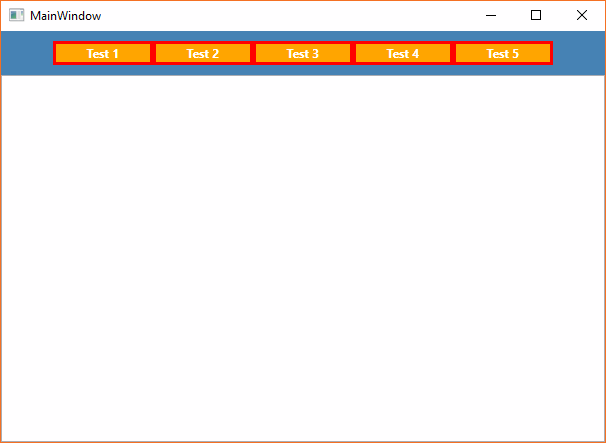
\includegraphics[width=1\textwidth]{resources_without.png}
\end{figure}

Предположим, что нам понадобилось изменить фон у кнопок на желтый, а обводку сделать тонкой красной линией. Здесь на помощь и приходят ресурсы. Обновим пример:

\begin{minted}{xml}
<Window x:Class="HelloWorldApp.MainWindow"
        xmlns="http://schemas.microsoft.com/winfx/2006/xaml/presentation"
        xmlns:x="http://schemas.microsoft.com/winfx/2006/xaml"
        xmlns:d="http://schemas.microsoft.com/expression/blend/2008"
        xmlns:mc="http://schemas.openxmlformats.org/markup-compatibility/2006"
        xmlns:local="clr-namespace:HelloWorldApp"
        xmlns:system="clr-namespace:System;assembly=mscorlib"
        mc:Ignorable="d"
        Title="MainWindow" Height="450" Width="620">

    <Window.Resources>
        <SolidColorBrush x:Key="ButtonBackgroundBrush">Yellow</SolidColorBrush>
        <SolidColorBrush x:Key="ButtonForegroundBrush">Red</SolidColorBrush>
        <SolidColorBrush x:Key="ButtonBorderBrush">Red</SolidColorBrush>
        <Thickness x:Key="ButtonBorderThinkness">1</Thickness>
        <FontWeight x:Key="ButtonFontWeight">Light</FontWeight>
    </Window.Resources>
    
    <Grid>
        <DockPanel Background="SteelBlue">
            <StackPanel 
                DockPanel.Dock="Top" Orientation="Horizontal" 
                HorizontalAlignment="Center" Margin="10" >
                <Button
                    MinWidth="100" Content="Test 1" 
                    BorderBrush="{StaticResource ButtonBorderBrush}"
                    BorderThickness="{StaticResource ButtonBorderThinkness}"
                    Background="{StaticResource ButtonBackgroundBrush}"
                    Foreground="{StaticResource ButtonForegroundBrush}"
                    FontWeight="{StaticResource ButtonFontWeight}" />

                <Button
                    MinWidth="100" Content="Test 2" 
                    BorderBrush="{StaticResource buttonBorderBrush}"
                    BorderThickness="{StaticResource ButtonBorderThinkness}"
                    Background="{StaticResource ButtonBackgroundBrush}"
                    Foreground="{StaticResource ButtonForegroundBrush}"
                    FontWeight="{StaticResource ButtonFontWeight}" />

                <Button
                    MinWidth="100" Content="Test 3" 
                    BorderBrush="{StaticResource buttonBorderBrush}"
                    BorderThickness="{StaticResource ButtonBorderThinkness}"
                    Background="{StaticResource ButtonBackgroundBrush}"
                    Foreground="{StaticResource ButtonForegroundBrush}"
                    FontWeight="{StaticResource ButtonFontWeight}" />

                <Button
                    MinWidth="100" Content="Test 4" 
                    BorderBrush="{StaticResource buttonBorderBrush}"
                    BorderThickness="{StaticResource ButtonBorderThinkness}"
                    Background="{StaticResource ButtonBackgroundBrush}"
                    Foreground="{StaticResource ButtonForegroundBrush}"
                    FontWeight="{StaticResource ButtonFontWeight}" />

                <Button
                    MinWidth="100" Content="Test 5" 
                    BorderBrush="{StaticResource buttonBorderBrush}"
                    BorderThickness="{StaticResource ButtonBorderThinkness}"
                    Background="{StaticResource ButtonBackgroundBrush}"
                    Foreground="{StaticResource ButtonForegroundBrush}"
                    FontWeight="{StaticResource ButtonFontWeight}" />
            </StackPanel>
            <TextBox/>
        </DockPanel>
    </Grid>
</Window>
\end{minted}

Результат:
\begin{figure}[H]
\centering
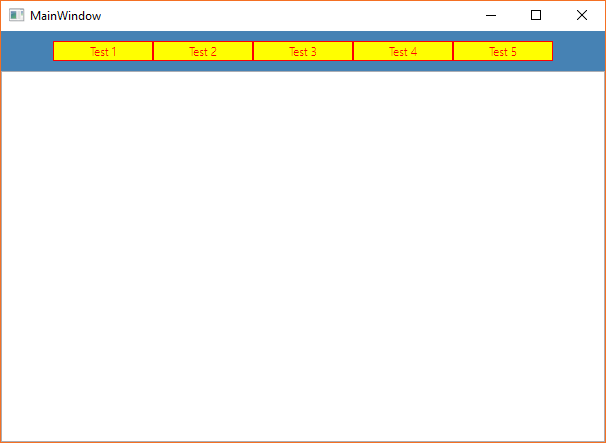
\includegraphics[width=1\textwidth]{resources_step1.png}
\end{figure}

Теперь мы можем отредактировать код только в 1 месте, чтобы изменить все кнопки. Попробуем применить стили, чтобы избавиться от дублирования:

\newpage

\begin{minted}{xml}
<Window x:Class="HelloWorldApp.MainWindow"
        xmlns="http://schemas.microsoft.com/winfx/2006/xaml/presentation"
        xmlns:x="http://schemas.microsoft.com/winfx/2006/xaml"
        xmlns:d="http://schemas.microsoft.com/expression/blend/2008"
        xmlns:mc="http://schemas.openxmlformats.org/markup-compatibility/2006"
        xmlns:local="clr-namespace:HelloWorldApp"
        xmlns:system="clr-namespace:System;assembly=mscorlib"
        mc:Ignorable="d"
        Title="MainWindow" Height="450" Width="620">

    <Window.Resources>
        <SolidColorBrush x:Key="ButtonBackgroundBrush">Yellow</SolidColorBrush>
        <SolidColorBrush x:Key="ButtonForegroundBrush">Red</SolidColorBrush>
        <SolidColorBrush x:Key="ButtonBorderBrush">Red</SolidColorBrush>

        <Thickness x:Key="ButtonBorderThinkness">1</Thickness>
        <FontWeight x:Key="ButtonFontWeight">Light</FontWeight>

        <Style TargetType="{x:Type Button}" x:Key="CustomButton">
            <Setter Property="Background" Value="{StaticResource ButtonBackgroundBrush}"/>
            <Setter Property="Foreground" Value="{StaticResource ButtonForegroundBrush}"/>
            <Setter Property="BorderBrush" Value="{StaticResource ButtonBorderBrush}"/>
            <Setter Property="BorderThickness" Value="{StaticResource ButtonBorderThinkness}"/>
            <Setter Property="FontWeight" Value="{StaticResource ButtonFontWeight}"/>
            <Setter Property="MinWidth" Value="100" />
        </Style>
    </Window.Resources>
    
    <Grid>
        <DockPanel Background="SteelBlue">
            <StackPanel 
                DockPanel.Dock="Top" Orientation="Horizontal" 
                HorizontalAlignment="Center" Margin="10" >
                <Button Style="{StaticResource CustomButton}" Content="Test 1" />
                <Button Style="{StaticResource CustomButton}" Content="Test 2" />
                <Button Style="{StaticResource CustomButton}" Content="Test 3" />
                <Button Style="{StaticResource CustomButton}" Content="Test 4" />
                <Button Style="{StaticResource CustomButton}" Content="Test 5" />
            </StackPanel>
            <TextBox/>
        </DockPanel>
    </Grid>
</Window>
\end{minted}

Результат аналогичен показанному выше, но мы получили решение, которое можно легко переиспользовать. Теперь создать кнопку с аналогичным стилем стало проще.


\subsubsection{Статические и динамические ресурсы}
В примерах выше мы использовали статические ресурсы (\mintinline{xml}{StaticResource}). Рассмотрим, для чего используются динамические ресурсы (\mintinline{xml}{DynamicResource}) и в чем заключаются их отличия. 

Итак, статические ресурсы устанавливается только один раз. А динамические ресурсы могут меняться в течение работы программы. Например, у нас есть ресурс кисти:

\begin{minted}{xml}
<SolidColorBrush Color="LightGray" x:Key="buttonBrush" />
\end{minted}

Для установки ресурса в качестве статического используется выражение \mintinline{xml}{StaticResource}:

\begin{minted}{xml}	
<Button 
    MaxWidth="80" MaxHeight="40" 
    Content="OK" Background="{StaticResource buttonBrush}" />
\end{minted}

Для установки ресурса как динамического применяется выражение \mintinline{xml}{DynamicResource}:

\begin{minted}{xml}
<Button 
    MaxWidth="80" MaxHeight="40" 
    Content="OK" Background="{DynamicResource buttonBrush}" />
\end{minted}

Причем один и тот же ресурс может быть и статическим и динамическим. Чтобы посмотреть различие между ними, добавим к кнопке обработчик нажатия:

\begin{minted}{xml}
<Button x:Name="button1" MaxWidth="80" MaxHeight="40" Content="OK"
        Background="{DynamicResource buttonBrush}"  Click="Button_Click" />
\end{minted}
        
А в файле кода определим в этом обработчике изменение ресурса:

\begin{minted}{csharp}
private void Button_Click(object sender, RoutedEventArgs e)
{
    this.Resources["buttonBrush"] = new SolidColorBrush(Colors.LimeGreen);
}
\end{minted}

И если после запуска мы нажмем на кнопку, то ресурс изменит свой цвет, что приведет к изменению цвета кнопки. Если бы ресурс был бы определен как статический, то изменение цвета кисти никак бы не повлияло на цвет фона кнопки.

В то же время надо отметить, что мы все равно может изменить статический ресурс - для этого нужно менять не сам объект по ключу, а его отдельные свойства:

\begin{minted}{csharp}
private void Button_Click(object sender, RoutedEventArgs e)
{
    // данное изменение будет работать и со статическими ресурсами
    SolidColorBrush buttonBrush = (SolidColorBrush)this.TryFindResource("buttonBrush");
    buttonBrush.Color = Colors.LimeGreen;
}
\end{minted}

% \paragraph{Иерархия ресурсов}

Еще одно различие между статическими и динамическими ресурсами касается поиска системой нужного ресурса. Так, при определении статических ресурсов ресурсы элемента применяются только к вложенным элементам, но не к внешним контейнерам. Например, ресурс кнопки мы не можем использовать для грида, а только для тех элементов, которые будут внутри этой кнопки. Поэтому, как правило, большинство ресурсов определяются в коллекции \mintinline{csharp}{Window.Resources} в качестве ресурсов всего окна, чтобы они были доступны для любого элемента данного окна.

В случае с динамическими ресурсами такого ограничения нет.

\subsubsection{Установка динамических ресурсов в коде C\texttt{\#}}

Ранее мы рассмотрели, как устанавливать в коде C\texttt{\#} статические ресурсы:

\begin{minted}{csharp}
LinearGradientBrush gradientBrush = new LinearGradientBrush();
gradientBrush.GradientStops.Add(new GradientStop(Colors.LightGray, 0));
gradientBrush.GradientStops.Add(new GradientStop(Colors.White, 1));
this.Resources.Add("buttonGradientBrush", gradientBrush);
 
button1.Background = (Brush)this.TryFindResource("buttonGradientBrush");
\end{minted}

Установка динамического ресурса призводится немного иначе:

\begin{minted}{csharp}
LinearGradientBrush gradientBrush = new LinearGradientBrush();
gradientBrush.GradientStops.Add(new GradientStop(Colors.LightGray, 0));
gradientBrush.GradientStops.Add(new GradientStop(Colors.White, 1));
this.Resources.Add("buttonGradientBrush", gradientBrush);
 
button1.SetResourceReference(Button.BackgroundProperty, "buttonGradientBrush");
\end{minted}

Для установки применяется метод \mintinline{csharp}{SetResourceReference()}, который есть у большинства элементов WPF. Первым параметром в него передается свойство зависимости объекта, для которого предназначен ресурс, а вторым — ключ ресурса.

\paragraph{Элементы \mintinline{xml}{StaticResource} и  \mintinline{xml}{DynamicResource}}

В ряде случае в разметке XAML бывает удобнее использовать не расширения разметки тип "{StaticResource}", а полноценные элементы DynamicResource и StaticResource. Например:

\begin{minted}{xml}
<Window x:Class="ResourcesApp.MainWindow"
        xmlns="http://schemas.microsoft.com/winfx/2006/xaml/presentation"
        xmlns:x="http://schemas.microsoft.com/winfx/2006/xaml"
        xmlns:d="http://schemas.microsoft.com/expression/blend/2008"
        xmlns:mc="http://schemas.openxmlformats.org/markup-compatibility/2006"
        xmlns:local="clr-namespace:ResourcesApp"
        mc:Ignorable="d"
        Title="Ресурсы" Height="250" Width="300">
    <Window.Resources>
        <SolidColorBrush Color="LimeGreen" x:Key="buttonBrush" />
    </Window.Resources>
    <Grid>
        <Button x:Name="button1" MaxWidth="80" MaxHeight="40" Content="OK">
            <Button.Background>
                <DynamicResource ResourceKey="buttonBrush" />
            </Button.Background>
        </Button>
    </Grid>
</Window>
\end{minted}

Элементы StaticResource и DynamicResource имеют свойство ResourceKey, которое позволяет установить ключ применяемого ресурса.

Особенно это эффективно может быть с контейнерами:

\begin{minted}{xml}
<Window x:Class="ResourcesApp.MainWindow"
        xmlns="http://schemas.microsoft.com/winfx/2006/xaml/presentation"
        xmlns:x="http://schemas.microsoft.com/winfx/2006/xaml"
        xmlns:d="http://schemas.microsoft.com/expression/blend/2008"
        xmlns:mc="http://schemas.openxmlformats.org/markup-compatibility/2006"
        xmlns:local="clr-namespace:ResourcesApp"
        mc:Ignorable="d"
        Title="Ресурсы" Height="250" Width="300">
    <Window.Resources>
        <Button x:Key="buttonRes" x:Shared="False" Content="OK" MaxHeight="40" MaxWidth="80" Background="Azure" />
    </Window.Resources>
    <StackPanel>
        <StaticResource ResourceKey="buttonRes" />
        <StaticResource ResourceKey="buttonRes" />
        <StaticResource ResourceKey="buttonRes" />
        <StaticResource ResourceKey="buttonRes" />
    </StackPanel>
</Window>
\end{minted}

\subsubsection{Словари ресурсов}

Мы можем определять ресурсы на уровне отдельных элементов окна, например, как ресурсы элементов Window, Grid и т.д. Однако есть еще один способ определения ресурсов, который предполагает использование словаря ресурсов.

Нажмем правой кнопкой мыши на проект и в контекстном меню выберем Add -> New Item..., И в окне добавления выберем пункт Resource Dictionary (WPF):

Задаим ему навзание ExampleDictionary.xaml и нажмем кнопку ОК.

После этого в проект добавляется новый файл. Он представляет собой обычный xaml-файл с одним корневым элементом ResourceDictionary:

\begin{minted}{xml}
<ResourceDictionary xmlns="http://schemas.microsoft.com/winfx/2006/xaml/presentation"
                    xmlns:x="http://schemas.microsoft.com/winfx/2006/xaml"
                    xmlns:local="clr-namespace:ResourcesApp">
     
</ResourceDictionary>
\end{minted}

Изменим его код, добавив какой-нибудь ресурс:

\begin{minted}{xml}
<ResourceDictionary xmlns="http://schemas.microsoft.com/winfx/2006/xaml/presentation"
                    xmlns:x="http://schemas.microsoft.com/winfx/2006/xaml"
                    xmlns:local="clr-namespace:ResourcesApp">
    <LinearGradientBrush x:Key="buttonBrush">
        <GradientStopCollection>
            <GradientStop Color="White" Offset="0" />
            <GradientStop Color="Blue" Offset="1" />
        </GradientStopCollection>
    </LinearGradientBrush>
</ResourceDictionary>
\end{minted}

После определения файла ресурсов его надо подсоединить к ресурсам приложения. Для этого откроем файл App.xaml, который есть в проекте по умолчанию и изменим его:

\begin{minted}{xml}
<Application x:Class="ResourcesApp.App"
             xmlns="http://schemas.microsoft.com/winfx/2006/xaml/presentation"
             xmlns:x="http://schemas.microsoft.com/winfx/2006/xaml"
             xmlns:local="clr-namespace:ResourcesApp"
             StartupUri="MainWindow.xaml">
    <Application.Resources>
        <ResourceDictionary>
            <ResourceDictionary.MergedDictionaries>
                <ResourceDictionary Source="Dictionary1.xaml" />
            </ResourceDictionary.MergedDictionaries>
        </ResourceDictionary>
    </Application.Resources>
</Application>
\end{minted}

Элемент ResourceDictionary.MergedDictionaries здесь представляет колекцию объектов ResourceDictionary, то есть словарей ресурсов, которые добавляются к ресурсам приложения. Затем в любом месте приложения мы сможем сослаться на этот ресурс:

\begin{minted}{xml}
<Button Content="OK" MaxHeight="40" MaxWidth="80" Background="{StaticResource buttonBrush}" />
\end{minted}


При этом одновременно мы можем добавлять в коллекцию ресурсов приложения множество других словарей или параллельно с ними определять еще какие-либо ресурсы:

\begin{minted}{xml}
<Application x:Class="ResourcesApp.App"
             xmlns="http://schemas.microsoft.com/winfx/2006/xaml/presentation"
             xmlns:x="http://schemas.microsoft.com/winfx/2006/xaml"
             xmlns:local="clr-namespace:ResourcesApp"
             StartupUri="MainWindow.xaml">
    <Application.Resources>
        <ResourceDictionary>
            <ResourceDictionary.MergedDictionaries>
                <ResourceDictionary Source="Dictionary1.xaml" />
                <ResourceDictionary Source="Dictionary2.xaml" />
                <ResourceDictionary Source="ButtonStyles.xaml" />
                <SolidColorBrush Color="LimeGreen" x:Key="limeButton" />
            </ResourceDictionary.MergedDictionaries>
        </ResourceDictionary>
    </Application.Resources>
</Application>
\end{minted}

\paragraph{Загрузка словаря ресурсов}
Нам необязательно добавлять словарь ресурсов через ресурсы приложения. У объекта ResourceDictionary имеется свойство Source, через которое мы можем связать ресурсы конкретного элемента со словарем:

\begin{minted}{xml}
<Window x:Class="ResourcesApp.MainWindow"
        xmlns="http://schemas.microsoft.com/winfx/2006/xaml/presentation"
        xmlns:x="http://schemas.microsoft.com/winfx/2006/xaml"
        xmlns:d="http://schemas.microsoft.com/expression/blend/2008"
        xmlns:mc="http://schemas.openxmlformats.org/markup-compatibility/2006"
        xmlns:local="clr-namespace:ResourcesApp"
        mc:Ignorable="d"
        Title="Ресурсы" Height="250" Width="300">
    <Window.Resources>
        <ResourceDictionary Source="Dictionary1.xaml" />
    </Window.Resources>
    <Grid>
        <Button Content="OK" MaxHeight="40" MaxWidth="80" Background="{StaticResource buttonBrush}" />
    </Grid>
</Window>
\end{minted}

Также мы можем загружать словарь динамически в коде C\#. Так, загрузим в коде C\# вышеопределенный словарь:

\begin{minted}{csharp}
this.Resources = new ResourceDictionary() { Source = new Uri("pack://application:,,,/Dictionary1.xaml") };
\end{minted}

При динамической загрузке, если мы определяем ресурсы через xaml, то они должны быть динамическими:

\begin{minted}{xml}
<Button Content="OK" MaxHeight="40" MaxWidth="80" Background="{DynamicResource buttonBrush}" />
\end{minted}

\subsection{Стили и триггеры}

\subsubsection{Концепция и использование стилей}
    
Стили позволяют определить набор некоторых свойств и их значений, которые потом могут применяться к элементам в xaml. Стили хранятся в ресурсах и отделяют значения свойств элементов от пользовательского интерфейса. Также стили могут задавать некоторые аспекты поведения элементов с помощью триггеров. Аналогом стилей могут служить каскадные таблицы стилей (CSS), которые применяются в коде html на веб-страницах.

Зачем нужны стили? Стили помогают создать стилевое единообразие для определенных элементов. Допустим, у нас есть следующий код xaml:

\begin{minted}{xml}
<StackPanel x:Name="buttonsStack" Background="Black" >
    <Button x:Name="button1" Margin="10" Content="Кнопка 1" FontFamily="Verdana" Foreground="White" Background="Black" />
    <Button x:Name="button2" Margin="10" Content="Кнопка 2" FontFamily="Verdana" Foreground="White" Background="Black"/>
</StackPanel>
\end{minted}

Здесь обе кнопки применяют ряд свойств с одними и теми же значениями:
\todo{Картинка}

Однако в данном случае мы вынуждены повторяться. Частично, проблему могло бы решить использование ресурсов:

\begin{minted}{xml}
<Window x:Class="StylesApp.MainWindow"
        xmlns="http://schemas.microsoft.com/winfx/2006/xaml/presentation"
        xmlns:x="http://schemas.microsoft.com/winfx/2006/xaml"
        xmlns:d="http://schemas.microsoft.com/expression/blend/2008"
        xmlns:mc="http://schemas.openxmlformats.org/markup-compatibility/2006"
        xmlns:local="clr-namespace:StylesApp"
        mc:Ignorable="d"
        Title="Стили" Height="250" Width="300">
    <Window.Resources>
        <FontFamily x:Key="buttonFont">Verdana</FontFamily>
        <SolidColorBrush Color="White" x:Key="buttonFontColor" />
        <SolidColorBrush Color="Black" x:Key="buttonBackColor" />
        <Thickness x:Key="buttonMargin" Bottom="10" Left="10" Top="10" Right="10" />
    </Window.Resources>
    <StackPanel x:Name="buttonsStack" Background="Black" >
        <Button x:Name="button1" Content="Кнопка 1"
                Margin="{StaticResource buttonMargin}"
                FontFamily="{StaticResource buttonFont}"
                Foreground="{StaticResource buttonFontColor}"
                Background="{StaticResource buttonBackColor}" />
        <Button x:Name="button2" Content="Кнопка 2"
                Margin="{StaticResource buttonMargin}"
                FontFamily="{StaticResource buttonFont}"
                Foreground="{StaticResource buttonFontColor}"
                Background="{StaticResource buttonBackColor}"/>
    </StackPanel>
</Window>
\end{minted}

Однако в реальности код раздувается, опть же приходится писать много повторяющейся информации. И в этом плане стили предлагают более элегантное решение:

\begin{minted}{xml}
<Window x:Class="StylesApp.MainWindow"
        xmlns="http://schemas.microsoft.com/winfx/2006/xaml/presentation"
        xmlns:x="http://schemas.microsoft.com/winfx/2006/xaml"
        xmlns:d="http://schemas.microsoft.com/expression/blend/2008"
        xmlns:mc="http://schemas.openxmlformats.org/markup-compatibility/2006"
        xmlns:local="clr-namespace:StylesApp"
        mc:Ignorable="d"
        Title="Стили" Height="250" Width="300">
    <Window.Resources>
        <Style x:Key="BlackAndWhite">
            <Setter Property="Control.FontFamily" Value="Verdana" />
            <Setter Property="Control.Background" Value="Black" />
            <Setter Property="Control.Foreground" Value="White" />
            <Setter Property="Control.Margin" Value="10" />
        </Style>
    </Window.Resources>
    <StackPanel x:Name="buttonsStack" Background="Black" >
        <Button x:Name="button1" Content="Кнопка 1"
                Style="{StaticResource BlackAndWhite}" />
        <Button x:Name="button2" Content="Кнопка 2"
                Style="{StaticResource BlackAndWhite}"/>
    </StackPanel>
</Window>
\end{minted}


Результат будет тот же, однако теперь мы избегаем не нужного повторения. Более того теперь мы можем управлять всеми нужными нам свойствами как единым целым - одним стилем.

Стиль создается как ресурс с помощью объекта Style, который представляет класс System.Windows.Style. И как любой другой ресурс, он обязательно должен иметь ключ. С помощью коллекции Setters определяется группа свойств, входящих в стиль. В нее входят объекты Setter, которые имеют следующие свойства:

Property: указывает на свойство, к которому будет применять данный сеттер. Имеет следующий синтаксис: Property="Тип\_элемента.Свойство\_элемента". Выше в качестве типа элемента использовался Control, как общий для всех элементво. Поэтому данный стиль мы могли бы применить и к Button, и к TextBlock, и к другим элементам. Однако мы можем и конкретизировать элемент, например, Button:

\begin{minted}{xml}
<Setter Property="Button.FontFamily" Value="Arial" />
\end{minted}

Value: устанавливает значение

Если значение свойства представляет сложный объект, то мы можем его вынести в отдельный элемент:

\begin{minted}{xml}
<Style x:Key="BlackAndWhite">
    <Setter Property="Control.Background">
        <Setter.Value>
            <LinearGradientBrush>
                <LinearGradientBrush.GradientStops>
                    <GradientStop Color="White" Offset="0" />
                    <GradientStop Color="Black" Offset="1" />
                </LinearGradientBrush.GradientStops>
            </LinearGradientBrush>
        </Setter.Value>
    </Setter>
    <Setter Property="Control.FontFamily" Value="Verdana" />
    <Setter Property="Control.Foreground" Value="White" />
    <Setter Property="Control.Margin" Value="10" />
</Style>
\end{minted}


\paragraph{TargetType}
Hам необязательно прописывать для всех кнопок стиль. Мы можем в самом определении стиля с помощью свойства TargetType задать тип элементов. В этом случае стиль будет автоматически применяться ко всем кнопкам в окне:

\begin{minted}{xml}
<Window x:Class="StylesApp.MainWindow"
        xmlns="http://schemas.microsoft.com/winfx/2006/xaml/presentation"
        xmlns:x="http://schemas.microsoft.com/winfx/2006/xaml"
        xmlns:d="http://schemas.microsoft.com/expression/blend/2008"
        xmlns:mc="http://schemas.openxmlformats.org/markup-compatibility/2006"
        xmlns:local="clr-namespace:StylesApp"
        mc:Ignorable="d"
        Title="Стили" Height="250" Width="300">
    <Window.Resources>
        <Style TargetType="Button">
            <Setter Property="FontFamily" Value="Verdana" />
            <Setter Property="Background" Value="Black" />
            <Setter Property="Foreground" Value="White" />
            <Setter Property="Margin" Value="10" />
        </Style>
    </Window.Resources>
    <StackPanel x:Name="buttonsStack" Background="Black" >
        <Button x:Name="button1" Content="Кнопка 1"  />
        <Button x:Name="button2" Content="Кнопка 2" />
    </StackPanel>
</Window>
\end{minted}


Причем в этом случае нам уже не надо указывать у стиля ключ x:Key несмотря на то, что это ресурс.

Также если используем свойство TargetType, то в значении атрибута Property уже необязательно указывать тип, то есть Property="Control.FontFamily". И в данном случае тип можно просто опустить: Property="FontFamily"

Если же необходимо, чтобы к какой-то кнопке не применялся автоматический стиль, то ее стилю присваивают значение null

\begin{minted}{xml}
<Button x:Name="button2" Content="Кнопка 2" Style="{x:Null}" />
\end{minted}

\paragraph{Определение обработчиков событий с помощью стилей}
Кроме коллекции Setters стиль может определить другую коллекцию - EventSetters, которая содержит объекты EventSetter. Эти объекты позволяют связать события элементов с обработчиками. Например, подключим все кнопки к одному обработчику события Click:

\begin{minted}{xml}
<Style TargetType="Button">
    <Setter Property="Button.Background" Value="Black" />
    <Setter Property="Button.Foreground" Value="White" />
    <Setter Property="Button.FontFamily" Value="Andy" />
    <EventSetter Event="Button.Click" Handler="Button_Click" />
</Style>
\end{minted}


Соответственно в файле кода C\# у нас должен быть определен обработчик Button\_Click:

\begin{minted}{csharp}
private void Button_Click(object sender, RoutedEventArgs e)
{
    Button clickedButton = (Button)sender;
    MessageBox.Show(clickedButton.Content.ToString());
}
\end{minted}


\paragraph{Наследование стилей и свойство BasedOn}

У класса Style еще есть свойство BasedOn, с помощью которого можно наследовать и расширять существующие стили:

\begin{minted}{xml}
<Window.Resources>
    <Style x:Key="ButtonParentStyle">
        <Setter Property="Button.Background" Value="Black" />
        <Setter Property="Button.Foreground" Value="White" />
        <Setter Property="Button.FontFamily" Value="Andy" />
    </Style>
    <Style x:Key="ButtonChildStyle" BasedOn="{StaticResource ButtonParentStyle}">
        <Setter Property="Button.BorderBrush" Value="Red" />
        <Setter Property="Button.FontFamily" Value="Verdana" />
    </Style>
</Window.Resources>
\end{minted}


Cвойство BasedOn в качестве значения принимает существующий стиль, определяя его как статический ресурс. В итоге он объединяет весь функционал родительского стиля со своим собственным.

Если в дочернем стиле есть сеттеры для свойств, которые также используются в родительском стиле, как в данном случае сеттер для свойства Button.FontFamily, то дочерний стиль переопределяет родительский стиль.

\subsection{Анимация}

\subsubsection{Использование анимаций в XAML}

Для определения анимации в XAML применяется объект EventTrigger или триггер событий. Этот объект имеет свойство Actions, которое определяет ряд действий, возникающих в результате генерации события. Само возникающее действие описывается через элемент BeginStoryboard, который и запускает анимацию.

Непосредственно для определения анимации используется объект Storyboard. Он объявляет объект анимации со всеми ее свойствами и параметрами. Например, проанимируем ширину кнопки:

\begin{minted}{xml}
<Window x:Class="AnimationApp.MainWindow"
        xmlns="http://schemas.microsoft.com/winfx/2006/xaml/presentation"
        xmlns:x="http://schemas.microsoft.com/winfx/2006/xaml"
        xmlns:d="http://schemas.microsoft.com/expression/blend/2008"
        xmlns:mc="http://schemas.openxmlformats.org/markup-compatibility/2006"
        xmlns:local="clr-namespace:AnimationApp"
        mc:Ignorable="d"
        Title="MainWindow" Height="250" Width="300">
    <Window.Triggers>
        <EventTrigger RoutedEvent="Loaded">
            <EventTrigger.Actions>
                <BeginStoryboard>
                    <Storyboard TargetProperty="Width" TargetName="helloButton">
                        <DoubleAnimation From="70" To="150"
                                         AutoReverse="True"
                                         RepeatBehavior="0:0:10"
                                         Duration="0:0:3"
                                         Completed="ButtonAnimation_Completed" />
                    </Storyboard>
                </BeginStoryboard>
            </EventTrigger.Actions>
        </EventTrigger>
    </Window.Triggers>
    <Grid>
        <Button x:Name="helloButton" Width="70" Height="30" Content="Hello" />
    </Grid>
</Window>
\end{minted}

У объекта EventTrigger с помощью атрибута RoutedEvent определяется событие, которое будет запускать анимацию. В данном случае это событие Loaded - загрузка окна.

Ряд настроек анимации устанавливает элемент Storyboard: TargetName задает анимируемый элемент, а TargetProperty определяет свойство элемента, которое будет анимироваться.

В принципе эти настройки также можно было бы вынести в объект анимации в виде прикрепляемых свойств:

\begin{minted}{xml}
<Storyboard>
    <DoubleAnimation Storyboard.TargetProperty="Width" Storyboard.TargetName="helloButton"
                        From="70" To="150"  ...>
\end{minted}
                        
И далее в самом объекте Storyboard определяется объект анимации DoubleAnimation с рядом настроек. Все настройки в прицнипе тут те же, что использовались для анимации в прошлом примере. Правда, при определении значений свойств здесь есть некоторые отличия.

Так, свойство RepeatBehavior инициализируется временем - "0:0:10", которое будет повторяться анимация. Чтобы указать число повторов, структуру RepeatBehavior надо инициализировать так: RepeatBehavior="2x", где 2 - количество повторов, а x - просто префикс, указывающий, что речь идет о количестве итераций, без него бы число интерпретировалось как количество дней. Третий способ задания этого свойства - RepeatBehavior="Forever" - в этом случае анимация будет продолжаться все время работы приложения.

Например, ниже установлено RepeatBehavior="Forever", а свойство DecelerationRatio замедляет анимацию, что создает эффект подскока шара в верх, где он, достигая максимальной точки, теряет скорость, а при падении вновь ее увеличивает:

\begin{minted}{xml}
<Window x:Class="AnimationApp.MainWindow"
        xmlns="http://schemas.microsoft.com/winfx/2006/xaml/presentation"
        xmlns:x="http://schemas.microsoft.com/winfx/2006/xaml"
        xmlns:d="http://schemas.microsoft.com/expression/blend/2008"
        xmlns:mc="http://schemas.openxmlformats.org/markup-compatibility/2006"
        xmlns:local="clr-namespace:AnimationApp"
        mc:Ignorable="d"
        Title="MainWindow" Height="250" Width="300">
    <Window.Triggers>
        <EventTrigger RoutedEvent="Button.Click">
            <EventTrigger.Actions>
                <BeginStoryboard>
                    <Storyboard Timeline.DesiredFrameRate="60">
                        <DoubleAnimation Storyboard.TargetName="ball" Storyboard.TargetProperty="(Canvas.Bottom)"
                                 From="0" To="160" AutoReverse="True" Duration="0:0:2.5" RepeatBehavior="Forever"
                                 DecelerationRatio="1"/>
                    </Storyboard>
                </BeginStoryboard>
            </EventTrigger.Actions>
        </EventTrigger>
    </Window.Triggers>
    <Grid>
        <Grid.RowDefinitions>
            <RowDefinition />
            <RowDefinition Height="Auto" />
        </Grid.RowDefinitions>
        <Canvas Background="LightPink">
            <Ellipse Name="ball" Fill="Red" Stroke="Black"  Width="15" Height="15"
                        Canvas.Left="130" Canvas.Bottom="0" />
        </Canvas>
        <Button Width="70" Height="25" Content="Кнопка" Grid.Row="1" Margin="10" />
    </Grid>
</Window>
\end{minted}

В данном случае так как в EventTrigger в качестве события определено Button.Click, то анимация будет запускаться по нажатию на кнопку.

По умолчанию анимация вызывается 60 раз в секунду, однако с помощью прикрепленного свойства Timeline.DesiredFrameRate можно задать частоту кадров в секунду, как в предыдущем примере.

Анимация свойств вложенных объектов
Анимация может применяться и к свойствам вложенных объектов, которые являются свойствами, например:

\begin{minted}{xml}
<Ellipse Name="ball" Stroke="Black"  Width="20" Height="20" Canvas.Left="130" Canvas.Bottom="0">
    <Ellipse.Fill>
        <RadialGradientBrush RadiusX="1" RadiusY="1" GradientOrigin="0.3, 0.3">
            <GradientStop Color="White" Offset="0" />
            <GradientStop Color="Blue" Offset="1" />
        </RadialGradientBrush>
    </Ellipse.Fill>
    <Ellipse.Triggers>
        <EventTrigger RoutedEvent="Window.Loaded">
            <BeginStoryboard>
                <Storyboard>
                    <ColorAnimation Storyboard.TargetProperty="Fill.GradientStops[1].Color"
                            To="Yellow" Duration="0:0:8" AutoReverse="True"
                            RepeatBehavior="Forever" />
                </Storyboard>
            </BeginStoryboard>
        </EventTrigger>
    </Ellipse.Triggers>
</Ellipse>
\end{minted}

Здесь свойство Fill элемента Ellipse инициализируется кистью RadialGradientBrush, которая имеет коллекцию GradientStops. Анимация же применяется ко второму объекту коллекции и его свойству Color.

Комплексные анимации
С помощью объекта Storyboard можно создавать и более комплексные анимации. Например, сделаем кнопку, которая одновременно меняет ширину, длину и цвет:

\begin{minted}{xml}
<Button x:Name="helloButton" Foreground="White" Width="70" Height="25" Content="Кнопка">
    <Button.Background>
        <SolidColorBrush x:Name="buttonColor" Color="Black" />
    </Button.Background>
    <Button.Triggers>
        <EventTrigger RoutedEvent="Loaded">
            <EventTrigger.Actions>
                <BeginStoryboard>
                    <Storyboard>
                        <DoubleAnimation Storyboard.TargetProperty="Width" Storyboard.TargetName="helloButton"
                              From="80" To="150"  AutoReverse="True" RepeatBehavior="0:0:10" Duration="0:0:2"  />
                        <DoubleAnimation Storyboard.TargetProperty="Height" Storyboard.TargetName="helloButton"
                              From="30" To="100" AutoReverse="True" RepeatBehavior="0:0:10" Duration="0:0:2" />
                        <ColorAnimation Storyboard.TargetName="buttonColor" Storyboard.TargetProperty="Color"
                              From="{Binding ElementName=buttonColor, Path=Color}" To="Red"
                              AutoReverse="True" RepeatBehavior="0:0:10" Duration="0:0:2" />
                    </Storyboard>
                </BeginStoryboard>
            </EventTrigger.Actions>
        </EventTrigger>
    </Button.Triggers>
</Button>
\end{minted}

Определение анимации в стиле
При этом необязательно знать имя элемента для анимации, можно прикрепить анимацию ко всем элементам одного типа и установить ее через стиль:

\begin{minted}{xml}
<Window x:Class="AnimationApp.MainWindow"
        xmlns="http://schemas.microsoft.com/winfx/2006/xaml/presentation"
        xmlns:x="http://schemas.microsoft.com/winfx/2006/xaml"
        xmlns:d="http://schemas.microsoft.com/expression/blend/2008"
        xmlns:mc="http://schemas.openxmlformats.org/markup-compatibility/2006"
        xmlns:local="clr-namespace:AnimationApp"
        mc:Ignorable="d"
        Title="MainWindow" Height="250" Width="300">
    <Window.Resources>
        <Style TargetType="Button">
            <Style.Triggers>
                <EventTrigger RoutedEvent="Button.Click">
                    <EventTrigger.Actions>
                        <BeginStoryboard>
                            <Storyboard>
                                <ColorAnimation Storyboard.TargetProperty="Background.Color"
                                        To="Red" AutoReverse="True" Duration="0:0:2" />
                            </Storyboard>
                        </BeginStoryboard>
                    </EventTrigger.Actions>
                </EventTrigger>
            </Style.Triggers>
        </Style>
    </Window.Resources>
    <StackPanel>
        <Button Width="70" Height="25" Content="Кнопка 1" Margin="10" />
        <Button Width="70" Height="25" Content="Кнопка 2" Margin="10" />
    </StackPanel>
</Window>
\end{minted}

Так как у стиля задан атриубут TargetType="Button", то анимация внутри триггера будет применяться ко всем кнопкам. В качестве анимируемого свойства указывается "Background.Color". То есть у класса Button есть свойство Background, представленное объектом SolidColorBrush, а у этого объекта есть свойство Color. Напрямую анимировать свойство Background мы не можем, так как ColorAnimation требует типа Color.

Так как стиль применяется глобально к кнопкам, то в настройках анимации название анимируемого элемента не указывается. Также не указывается свойство From, а это значит, что анимация будет идти от текущего цвета кнопки.

Теперь после нажатия натажатая кнопка будет ненадолго окрашиваться в красный, а затем возвращать исходный цвет.

\subsection{Работа с графикой}

\subsubsection{Фигуры}

Одним из способов построения двухмерной графики в окне - это использование фигур. Фигуры фактически являются обычными элементами как например кнопка или текстовое поле. К фигурам относят такие элементы как Polygon (Многоугольник), Ellipse (овал), Rectangle (прямоугольник), Line (обычная линия), Polyline (несколько связанных линий). Все они наследуются от абстрактного базового класса System.Windows.Shapes.Shape:

От базового класса они наследуют ряд общих свойств:

Fill заполняет фон фигуры с помощью кисти - аналогичен свойству Background у прочих элементов
Stroke задает кисть, которая отрисовывает границу фигуры - аналогичен свойству BorderBrush у прочих элементов
StrokeThikness задает толщину границы фигуры - аналогичен свойству BorderThikness у прочих элементов
StrokeStartLineCap и StrokeEndLineCap задают для незамкнутых фигур (Line) контур в начале и в конце линии соответственно
StrokeDashArray задает границу фигуры в виде штриховки, создавая эффект пунктира
StrokeDashOffset задает расстояние до начала штриха
StrokeDashCap задает форму штрихов

\paragraph{Ellipse}
Ellipse представляет овал:

\begin{minted}{xml}
<Ellipse Fill="LightBlue" Width="200" Height="200" />
\end{minted}

При одинаковой ширине и высоту получается круг:

\paragraph{Ellipse}

Rectangle представляет прямоугольник::

\begin{minted}{xml}
<StackPanel Background="White">
    <Rectangle Fill="LightBlue" Width="200" Height="100" Margin="10" />
    <Rectangle Fill="LightPink" Width="200" Height="100" RadiusX="15" RadiusY="15" Margin="10" />
</StackPanel>
\end{minted}

С помощью свойств RadiusX и RadiusY можно округлить углы прямоугольника:

\paragraph{Line}

Line представляет простую линию. Для создания линии надо указать координаты в ее свойствах X1, Y1, X2 и Y2. При этом надо учитывать, что началом координатной системы является верхний левый угол:

\begin{minted}{xml}
<Line X1="100" Y1="30" X2="200" Y2="150" Stroke="Red" />
<Line X1="100" Y1="150" X2="200" Y2="30" Stroke="Blue" />
\end{minted}

\paragraph{Polygon}

Polygon представляет многоугольник. С помощью коллекции Points элемент устанавливает набор точек - объектов типа Point, которые последовательно соединяются линиями, причем последня точка соединяется с первой:

\begin{minted}{xml}
<Polygon Fill="LightPink" Points="50, 150, 150, 50, 250, 150" />
\end{minted}

В данном случае у нас три точки (50, 150), (150, 50) и (250, 150), которые образуют треугольник.

\paragraph{Polyline}

Polyline представляет набор точек, соединенных линиями. В этом плане данный элемент похож на Polygon за тем исключением, что первая и последняя точка не соединяются:

\begin{minted}{xml}
<Polyline Stroke="Red" Points="50, 150, 150, 50, 250, 150" />
\end{minted}

\subsubsection{Пути и геометрии}

Фигуры удобны для создания самых простейших рисунков, дизайна, однако что-то более сложное и комплексное с их помощью сделать труднее. Поэтому для этих целей применяется класс Path, который представляет геометрический путь. Он также, как и фигуры, наследуется от класса Shape, но может заключать в себе совокупность объединенных фигур. Класс Path имеет свойство Data, которое определяет объект Geometry - геометрический объект для отрисовки. Этот объект задает фигуру или совукупность фигур для отрисовки.

Класс Geometry - абстрактный, поэтому в качестве объекта используется один из производных классов:

LineGeometry представляет линию, эквивалент фигуры Line

RectangleGeometry представляет прямоугольник, эквивалент фигуры Rectangle

EllipseGeometry представляет эллипс, эквивалент фигуры Ellipse

PathGeometry представляет путь, образующий сложную геометрическую фигуру из простейших фигур

GeometryGroup создает фигуру, состоящую из нескольких объектов Geometry

CombinedGeometry создает фигуру, состоящую из двух объектов Geometry

StreamGeometry - специальный объект Geometry, предназначенный для сохранения всего геометрического пути в памяти

\paragraph{LineGeometry}
Например, использование LineGeometry:

\begin{minted}{xml}
<Path Stroke="Blue">
    <Path.Data>
        <LineGeometry StartPoint="100,30" EndPoint="200,130" />
    </Path.Data>
</Path>
\end{minted}

будет аналогично следующему объекту Line:

\begin{minted}{xml}
<Line X1="100" Y1="30" X2="200" Y2="130" Stroke="Blue" />
\end{minted}

Свойства StartPoint и EndPoint задают начальную и конечную точки линии.

\paragraph{RectangleGeometry}

\begin{minted}{xml}
<StackPanel>
    <Path Fill="LightBlue">
        <Path.Data>
            <RectangleGeometry Rect="100,20 100,50" />
        </Path.Data>
    </Path>
    <Path Fill="LightPink">
        <Path.Data>
            <RectangleGeometry Rect="100,20 100,50" RadiusX="10" RadiusY="10" />
        </Path.Data>
    </Path>
</StackPanel>
\end{minted}

Свойство Rect задает параметры прямоугольника в формате "координата X, координата Y ширина, высота". Также с помощью свойств RadiusX и RadiusY можно задать радиус скругления углов прямоугольника.

\paragraph{EllipseGeometry}

\begin{minted}{xml}
<Path Fill="LightPink" Stroke="LightBlue">
    <Path.Data>
        <EllipseGeometry RadiusX="50" RadiusY="25" Center="120,70" />
    </Path.Data>
</Path>
\end{minted}

Свойство Center устанавливает цетр овала, а свойста RadiusX и RadiusY - радиусы.

\paragraph{GeometryGroup}
GeometryGroup объединяет несколько геометрий:

\begin{minted}{xml}
<Path Fill="LightPink" Stroke="LightBlue">
    <Path.Data>
        <GeometryGroup  FillRule="Nonzero">
            <LineGeometry StartPoint="10,10" EndPoint="220,10" />
            <EllipseGeometry Center="100,100" RadiusX="50" RadiusY="40" />
            <RectangleGeometry Rect="120,100 80,20" RadiusX="5" RadiusY="5" />
        </GeometryGroup>
    </Path.Data>
</Path>
\end{minted}

Объект GeometryGroup устанавливает свойство FillRule. Если оно равно EvenOdd (значение по умолчанию), то перекрывающиеся поверхности двух геометрий являются прозрачными. А при значении FillRule="Nonzero" (как в данном случае), перекрывающиеся поверхности геометрий будут окрашены также, как и остальные части пути.

\paragraph{CombinedGeometry}
CombinedGeometry состоит из двух геометрий. В этом он похож на GeometryGroup, который также может объединять две геометрии. Однако между ними есть различия. Отличие состоит в том, что объект CombinedGeometry имеет свойство GeometryCombinedMode, которое указывает модель перекрытия двух геометрий:

Union: фигура включает обе геометрии

Intersect: фигура включает область, которая одновременно принадлежит обеим геометриям

Xor: фигура включает только непересекающие области геометрий

Exclude: фигура включает первую геометрию с исключением тех областей, которые принадлежат также и второй геометрии

Применим все способы:

\begin{minted}{xml}
<Grid>
    <Grid.RowDefinitions>
        <RowDefinition />
        <RowDefinition />
        <RowDefinition />
        <RowDefinition />
    </Grid.RowDefinitions>
    <Path Fill="LightPink" Stroke="LightBlue">
        <Path.Data>
            <CombinedGeometry GeometryCombineMode="Union">
                <CombinedGeometry.Geometry1>
                    <EllipseGeometry Center="50,60" RadiusX="50" RadiusY="50" />
                </CombinedGeometry.Geometry1>
                <CombinedGeometry.Geometry2>
                    <RectangleGeometry Rect="60, 20 120,80" />
                </CombinedGeometry.Geometry2>
            </CombinedGeometry>
        </Path.Data>
    </Path>
    <Path Grid.Row="1" Fill="LightPink" Stroke="LightBlue">
        <Path.Data>
            <CombinedGeometry GeometryCombineMode="Xor">
                <CombinedGeometry.Geometry1>
                    <EllipseGeometry Center="50,60" RadiusX="50" RadiusY="50" />
                </CombinedGeometry.Geometry1>
                <CombinedGeometry.Geometry2>
                    <RectangleGeometry Rect="60, 20 120,80" />
                </CombinedGeometry.Geometry2>
            </CombinedGeometry>
        </Path.Data>
    </Path>
    <Path Grid.Row="2" Fill="LightPink" Stroke="LightBlue">
        <Path.Data>
            <CombinedGeometry GeometryCombineMode="Intersect">
                <CombinedGeometry.Geometry1>
                    <EllipseGeometry Center="50,60" RadiusX="50" RadiusY="50" />
                </CombinedGeometry.Geometry1>
                <CombinedGeometry.Geometry2>
                    <RectangleGeometry Rect="60, 20 120,80" />
                </CombinedGeometry.Geometry2>
            </CombinedGeometry>
        </Path.Data>
    </Path>
    <Path Grid.Row="3" Fill="LightPink" Stroke="LightBlue">
        <Path.Data>
            <CombinedGeometry GeometryCombineMode="Exclude">
                <CombinedGeometry.Geometry1>
                    <EllipseGeometry Center="50,60" RadiusX="50" RadiusY="50" />
                </CombinedGeometry.Geometry1>
                <CombinedGeometry.Geometry2>
                    <RectangleGeometry Rect="60, 20 120,80" />
                </CombinedGeometry.Geometry2>
            </CombinedGeometry>
        </Path.Data>
    </Path>
</Grid>
\end{minted}

\subsubsection{Трансформации}

Трансформации представляют инструмент изменения положения или размера элементов WPF. Трансформации могут быть полезны в тех ситуациях, когда надо изменить положение элемента, либо анимировать. Все трансформации наследуются от абстрактного базового класса System.Windows.Media.Transform и представляют следующие классы:

TranslateTransform: сдвигает элементы по горизонтали и вертикали
RotateTransform: вращает элемент
ScaleTransform: выполняет операции масштабирования
SkewTransform: изменяет позицию элемента путем наклона на определенное количество градусов
MatrixTransform: изменяет координатную систему в соответствии с определенной матрицей
TransformGroup: представляет группу трансформаций

\paragraph{RotateTransform}

RotateTransform поворачивает элемент вокруг оси на определенное количество градусов. Данный объект принимает три основых параметра:
Angle: угол поворота
CenterX: устанавливает центр вращения по оси X
CenterY: устанавливает центр вращения по оси Y

\begin{minted}{xml}
<Rectangle Width="100" Height="30" Stroke="Blue" Fill="LightBlue">
    <Rectangle.RenderTransform>
        <RotateTransform Angle="45" />
    </Rectangle.RenderTransform>
</Rectangle>
\end{minted}

\paragraph{TranslateTransform}
TranslateTransform позволяет сместить положение элемента по оси X, с помощью свойства X, и по оси Y - с помощью свойства Y.

\begin{minted}{xml}
<Rectangle Width="100" Height="30" Stroke="Blue" Fill="LightBlue">
    <Rectangle.RenderTransform>
        <TranslateTransform X="20" Y="-30" />
    </Rectangle.RenderTransform>
</Rectangle>
\end{minted}

\paragraph{ScaleTransform}
Обеспечивает масштабирование элемента на определенную величину. Для изменения ширины надо задать свойство ScaleX, а для изменения длины - свойство ScaleY. Кроме того, также имеются свойства CenterX и CenterY, позволяющие позиционировать элемент.

Например, увеличение прямоугольника в полтора раза:

\begin{minted}{xml}
<Rectangle Width="100" Height="30" Stroke="Blue" Fill="LightBlue">
    <Rectangle.RenderTransform>
        <ScaleTransform ScaleX="1.5" ScaleY="1.5" />
    </Rectangle.RenderTransform>
</Rectangle>
\end{minted}

\paragraph{SkewTransform}
SkewTransform позволяет задать наклон элемента вдоль оси X с помощью свойства AngleX, и по оси Y - с помощью свойства AngleY. А с помощью свойств CenterX и CenterY можно изменить положение элемента относительно осй X и Y:

\begin{minted}{xml}
<Rectangle Width="100" Height="30" Stroke="Blue" Fill="LightBlue">
    <Rectangle.RenderTransform>
        <SkewTransform AngleX="45"  />
    </Rectangle.RenderTransform>
</Rectangle>
\end{minted}

\paragraph{MatrixTransform}
Осуществляет матричное преобразование элемента. В свойстве Matrix мы задаем первые два столбца, которые применяются при преобразовании. Последний столбец по умолчанию имеет значения {0 0 1}.

\begin{minted}{xml}
<Rectangle Width="100" Height="30" Stroke="Blue" Fill="LightBlue">
    <Rectangle.RenderTransform>
        <MatrixTransform Matrix="1 0 1 2 1 -3" />
    </Rectangle.RenderTransform>
</Rectangle>
\end{minted}

\paragraph{TransformGroup}
TransformGroup позволяет комбинировать различные трансформации вместе:

\begin{minted}{xml}
<Rectangle Width="100" Height="30" Stroke="Blue" Fill="LightBlue">
    <Rectangle.RenderTransform>
        <TransformGroup>
            <RotateTransform Angle="45" />
            <TranslateTransform Y="-40" X="30" />
        </TransformGroup>
    </Rectangle.RenderTransform>
</Rectangle>
\end{minted}

\paragraph{RenderTransform и LayoutTransform}
Для применения трансформаций у фигур и стандартных элементов управления WPF используются свойства RenderTransform и LayoutTransform. Несмотря на то, что для обоих свойств трансформации задаются одинаково, их действие различается. Так, свойство LayoutTransform применяется до компоновки элемента, а RenderTransform - после, поэтому одинаковые трансформации для этих свойств могут давать немного разные результаты:

\begin{minted}{xml}
<Grid>
    <Grid.ColumnDefinitions>
        <ColumnDefinition />
        <ColumnDefinition />
    </Grid.ColumnDefinitions>
    <Button Width="80" Height="30" Background="LightBlue" Content="Hello">
        <Button.RenderTransform>
            <RotateTransform Angle="-45" />
        </Button.RenderTransform>
    </Button>
    <Button Grid.Column="1" Width="80" Height="30" Background="LightBlue" Content="Hello">
        <Button.LayoutTransform>
            <RotateTransform Angle="-45" />
        </Button.LayoutTransform>
    </Button>
</Grid>
\end{minted}

\todo{Перенести это все на момент после главы data}
\subsection{Разработка элементов управления и их логики}

\subsubsection{Класс DependencyObject. Введение в Dependency Property}

До этого мы рассматривали базовые компоненты WPF и их основные свойства. Однако рассмотренные свойства элементов, как например, Width или Height, являются не просто стандартными свойствами языка C#. Они фактически скрывают свойства зависимостей или dependency property. Без свойств зависимостей были бы невозможны многие ключевые особенности WPF, как привязка данных, стили, анимация и т.д.

Рассмотрим, как они определяются. Возьмем, к примеру, элемент TextBlock, у которого есть свойство Text:

public class TextBlock : FrameworkElement, IContentHost, IAddChildInternal, IServiceProvider 
{
    // свойство зависимостей
    public static readonly DependencyProperty TextProperty;
 
    static TextBlock()
    {
        // Регистрация свойства
        TextProperty = DependencyProperty.Register(
                    "Text", 
                    typeof(string),
                    typeof(TextBlock),
                    new FrameworkPropertyMetadata(
                        string.Empty, 
                        FrameworkPropertyMetadataOptions.AffectsMeasure |
                        FrameworkPropertyMetadataOptions.AffectsRender, 
                        new PropertyChangedCallback(OnTextChanged), 
                        new CoerceValueCallback(CoerceText)));
        // остальной код
    }
 
    // Обычное свойство .NET  - обертка над свойством зависимостей
    public string Text
    { 
        get { return (string) GetValue(TextProperty); } 
        set { SetValue(TextProperty, value); }
    }  
     
    private static object CoerceText(DependencyObject d, object value)
    {
        //.................................
    }
    // метод, вызываемый при изменении значения свойства 
    private static void OnTextChanged(DependencyObject d, DependencyPropertyChangedEventArgs e)
    { 
        //...............................
    }
    // остальной код
}

Статическое свойство TextProperty является свойством зависимостей, представляя объект System.Windows.DependencyProperty. По соглашениям по именованию все свойства зависимостей представляют статические публичные поля (public static) с суффиксом Property.

Затем в статическом конструкторе класса происходит регистрация свойства с помощью метода DependencyProperty.Register(), в который передается ряд параметров:

имя свойства (в данном случае "Text"). Как правило, соответствует названию свойства зависимостей без суффикса Property

тип свойства (в данном случае string)

тип, который владеет свойством - собственно тот тип, в котором свойство определено или в данном случае тип TextBlock

Необязательный параметр FrameworkPropertyMetadata устанавливает дополнительные настройки свойства

В качестве пятого необязательного параметра может использоваться ссылка на метод, который производит валидацию свойства. В данном случае этот параметр опущен.

Первые три обязательных свойства довольно просты, поэтому подробнее остановимся на четвертом необязательном параметре, представляющем объект FrameworkPropertyMetadata. Данный объект содержит ряд свойств для конфигурации свойства зависимостей:

AffectsArrange: если имеет значение true, то свойство зависимостей будет влиять на процесс компоновки элемента

AffectsMeasure: если имеет значение true, то свойство зависимостей будет учитываться при установке размеров элемента при компоновке

AffectsParentArrange: если имеет значение true, то свойство зависимостей будет влиять на процесс компоновки в родительском элементе

AffectsParentMeasure: если имеет значение true, то свойство зависимостей будет учитываться при установке размеров родительского элемента при его компоновке

AffectsRender: если имеет значение true, то свойство зависимостей будет влиять на рендеринг и визуализацию элемента

BindsTwoWayByDefault: если имеет значение true, то свойство зависимостей будет использовать двустороннюю привязку данных

CoerceValueCallback: хранит ссылку на метод, который применяется для проверки допустимости значения до его валидации. Если значение не допустимо, то оно может корректироваться, чтобы соответствовать допустимым диапазонам.

DefaultValue: устанавливает значение по умолчанию для свойства зависимостей

Inherits: если имеет значение true, то вложенные элементы применительно к себе могут изменять значение свойства зависимостей. Например, если контейнер Windows задает свойство FontSize, то TextBlock автоматически подхватываетего значение, если в нем самом это свойство не установлено

IsAnimationProhibited: если имеет значение true, то свойство зависимостей не применяется при анимации

IsNotDataBindable: если имеет значение true, то свойство зависимостей не будет поддерживать привязку данных

Journal: если имеет значение true, то значение свойства зависимостей будет журналироваться (сохраняться)

PropertyChangedCallback: хранит ссылку на метод, который вызывается при изменении значения свойства

SubPropertiesDoNotAffectRender: если имеет значение true, то элемент не будет перерисовываться, если если какое-то подсвойства у свойства зависимостей изменит свое значение

В данном случае применяется один из конструкторов:

new FrameworkPropertyMetadata(string.Empty, 
    FrameworkPropertyMetadataOptions.AffectsMeasure | FrameworkPropertyMetadataOptions.AffectsRender, 
    new PropertyChangedCallback(OnTextChanged), new CoerceValueCallback(CoerceText)))
    
Этот конструктор устанавливает в качестве значени по умолчанию пустую строку, указывает, что при изменении значения элемент будет перерисовываться (собственно, что мы и видим - при изменении значения свойства Text новое значение отображается), и при изменении значения свойства будут вызываться методы OnTextChanged и CoerceText.

Далее после регистрации свойства идет обертка - обычное свойство .NET, которое имеет сеттер и геттер и которое вызывает методы GetValue и SetValue для получения и установки значения соответственно. Эти методы определены в классе System.Windows.DependencyObject, который является базовым для всех элементов WPF, в том числе и для TextBlock.

Последнее обстоятельство привносит ограничение - свойства зависимостей могут быть определены только в тех классах, которые наследутся от DependencyObject.

Кроме того, DependencyObject поддерживает еще ряд свойств для управления свойствами зависимостей:

ClearValue: очищает значение объекта DependencyProperty

InvalidateProperty: повторно вычисляет действующее значение объекта DependencyProperty

ReadLocalValue: считывает значение объекта DependencyProperty

Пример:
someTextBlock.Text = "Hello";
var text = (string) textBlock.ReadLocalValue(TextBlock.TextProperty); // Hello
someTextBlock.ClearValue(TextBlock.TextProperty); // теперь значение отсутствует


\subsubsection{Прикрепляемые свойства}

Прикрепляемые свойства (attached properties) также являются свойствами зависимостей с той разницей, что они определяются в одном классе, а применяются в другом. Например, при установке столбца или строки грида, в которых размещается элемент управления, используются свойства Grid.Row и Grig.Column, которые как раз и представляют прикрепляемые свойства. То есть эти свойства определены в классе Grid, но используются в других вложенных элементах:

<Grid>
    <Grid.RowDefinitions>
        <RowDefinition />
        <RowDefinition />
    </Grid.RowDefinitions>
    <Grid.ColumnDefinitions>
        <ColumnDefinition />
        <ColumnDefinition />
    </Grid.ColumnDefinitions>
    <Button x:Name="HelloButton" Content="Hello" Grid.Column="1" Grid.Row="0" />
</Grid>

В коде C# установка значения для прикрепленных свойств производится с помощью статических методов в формате Класс.Set[Свойство](). Например, установим для выше определенной кнопки столбец и строку грида:

Grid.SetRow(button1, 1); // вторая строка
Grid.SetColumn(button1, 1); // второй столбец

С помощью методов типа Класс.GetСвойство() мы можем получать в коде значения прикрепляемых свойств:

int column = Grid.GetColumn(button1); // получаем номер столбца


Если более детально взглянуть на прикрепляемые свойства, то можно увидеть, что их определение немного отличается от стандартных свойств зависимостей. Для регистрации прикрепляемого свойства применяется метод RegisterAttached():

Grid.ColumnProperty = DependencyProperty.RegisterAttached(
                        "Column", 
                        typeof(int), 
                        typeof(Grid), 
                        new FrameworkPropertyMetadata(0, 
                            new PropertyChangedCallback(Grid.OnCellAttachedPropertyChanged)), 
                        new ValidateValueCallback(Grid.IsIntValueNotNegative));
                        
Метод RegisterAttached() принимает те же параметры, что и метод Register().

Другое отличие от обычных свойств зависимостей состоит в том, что для прикрепляемых свойств не создается обертка в виде стандартного свойства C#. Вместо этого используется пара статических методов SetСвойство() GetСвойство():

public static int GetColumn(UIElement element)
{
    if (element == null)
    {
        throw new ArgumentNullException(...);
    }
    return (int)element.GetValue(Grid.ColumnProperty);
}
public static void SetColumn(UIElement element, int value)
{
    if (element == null)
    {
        throw new ArgumentNullException();
    }
    element.SetValue(Grid.ColumnProperty, value);
}

\subsubsection{Создание свойств}

Рассмотрим, как мы можем определять какие-то свои свойства зависимостей. Итак, определим в нашем проекте новый класс Phone:

public class Phone : DependencyObject
{
    public static readonly DependencyProperty TitleProperty;
    public static readonly DependencyProperty PriceProperty;
 
    static Phone()
    {
        TitleProperty = DependencyProperty.Register("Title", typeof(string), typeof(Phone));
        PriceProperty = DependencyProperty.Register("Price", typeof(int), typeof(Phone));
    }
    public string Title
    {
        get { return (string)GetValue(TitleProperty); }
        set { SetValue(TitleProperty, value); }
    }
    public int Price
    {
        get { return (int)GetValue(PriceProperty); }
        set { SetValue(PriceProperty, value); }
    }
}

Если мы хотим применять свойства зависимостей, то нам надо унаследовать свой класс от абстрактного класса DependencyObject. В нашем классе мы определяем два свойства зависимостей: TitleProperty и PriceProperty. Обратите внимание, что они объявляются с модификаторами public static readonly.

Затем свойства регистрируются в статическом конструкторе нашего класса с помощью метода Register. И в конце для них создаются обычные свойства-обертки, в которых мы получаем доступ к значению свойств с помощью методов GetValue и SetValue.

Теперь используем наш класс. Для этого определим следующую разметку XAML:

<Window x:Class="DependencyApp.MainWindow"
        xmlns="http://schemas.microsoft.com/winfx/2006/xaml/presentation"
        xmlns:x="http://schemas.microsoft.com/winfx/2006/xaml"
        xmlns:d="http://schemas.microsoft.com/expression/blend/2008"
        xmlns:mc="http://schemas.openxmlformats.org/markup-compatibility/2006"
        xmlns:local="clr-namespace:DependencyApp"
        mc:Ignorable="d"
        Title="MainWindow" Height="250" Width="300" FontSize="20">
    <Window.Resources>
        <local:Phone Price="600" Title="iPhone 6S" x:Key="iPhone6s" />
    </Window.Resources>
    <Grid x:Name="grid1" DataContext="{StaticResource iPhone6s}">
        <Grid.RowDefinitions>
            <RowDefinition />
            <RowDefinition />
            <RowDefinition />
        </Grid.RowDefinitions>
        <Grid.ColumnDefinitions>
            <ColumnDefinition />
            <ColumnDefinition />
        </Grid.ColumnDefinitions>
        <TextBlock Text="Модель" />
        <TextBlock Text="{Binding Title}" Grid.Column="1"  />
        <TextBlock Text="Цена" Grid.Row="1" />
        <TextBox Text="{Binding Price, Mode=TwoWay}" Grid.Column="1" Grid.Row="1"  />
        <Button Content="Check" Grid.Row="2" Grid.Column="2" Click="Button_Click" />
    </Grid>
</Window>

Здесь в ресурсах окна определяется объект Phone с установкой его свойств Price и Name:

	
<local:Phone Price="600" Title="iPhone 6S" x:Key="iPhone6s" />

Данный ресурс имеет ключ iPhone6s, по которому мы можем к нему обратиться. Далее для контейнера Grid мы задаем этот ресурс как контекст данных:

<Grid x:Name="grid1" DataContext="{StaticResource iPhone6s}">

Установка контекста данных позволяет внутри грида привязать отдельные элеметы к свойства ресурса, то есть объекта Phone:

<TextBox Text="{Binding Price, Mode=TwoWay}" Grid.Column="1" Grid.Row="1"  />


То же самое и для элемента TextBlock. Однако для TextBox у нас действует не просто привязка, а двусторонняя привязка, обозначенная параметром Mode=TwoWay. А это значит, что любые изменения свойства Price в ресурсе будут отображаться в текстовом поле. И наоборот - любые изменения в текстовом поле будут менять значения в ресурсе.

В этом состоит одно из преимуществ использования свойств зависимостей - для обычных свойств подобные привязки бы не работали.

Для проверки значения ресурса я добавил кнопку, у которой установил обработчик нажатия - Button_Click. И также добавим код этого обработчика в файл кода C#:

private void Button_Click(object sender, RoutedEventArgs e)
{
    Phone phone = (Phone)this.Resources["iPhone6s"]; // получаем ресурс по ключу
    MessageBox.Show(phone.Price.ToString());
}

Запустим приложение, изменим значение в текстовом поле, например, на 800 и нажмем на кнопку:

% \subsubsection{Создание своего компонента}

% Хороший способ начать разработку пользовательских элементов управления — попробовать создать самый простой элемент. В этом разделе мы начнем с создания базового указателя цвета.